\documentclass[border=4pt]{standalone}
\usepackage{tikz}
\usetikzlibrary{arrows.meta,decorations.pathmorphing,positioning}
\begin{document}
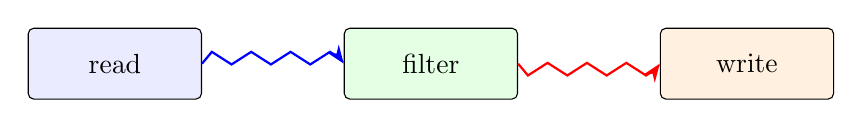
\begin{tikzpicture}[
  node distance=18mm,
  stage/.style={draw,rounded corners=2pt,minimum width=22mm,minimum height=9mm},
  signal/.style={-Stealth,thick,decorate,decoration={zigzag,segment length=5mm,amplitude=.8mm}}
]
  \node[stage,fill=blue!8] (read) {read};
  \node[stage,fill=green!10,right=of read] (filter) {filter};
  \node[stage,fill=orange!12,right=of filter] (write) {write};
  \draw[signal,blue,decoration={zigzag,segment length=5mm,amplitude=.8mm,raise=.7mm}]
    (read) -- (filter);
  \draw[signal,red,decoration={zigzag,segment length=5mm,amplitude=.8mm,mirror,raise=.7mm}]
    (filter) -- (write);
\end{tikzpicture}
\end{document}
